% Use class option [extendedabs] to prepare the 1-page extended abstract.
\documentclass[extendedabs]{bmvc2k}
\usepackage[colorlinks = true,
            linkcolor = blue,
            urlcolor  = blue,
            citecolor = blue,
            anchorcolor = blue]{hyperref}
\usepackage{kotex} % 한국어 사용 가능

% Document starts here
\begin{document}
\title{You Only Look Once : Unified, Real-Time Object Detection}
\addauthor{
Lee Gwan Hui$^1$, \today}{}{1}
\addinstitution{
$^1$2017142136, Department of Electrical and Electronic Engineering, Yonsei University.}
\maketitle
\let\thefootnote\relax\footnote{This is an extended abstract. The full paper is available at the \href{https://github.com/LeeGwanHui/TIL/tree/main/deeplearning_ham}{github}. }
\vspace{-0.2in}

\section{Object Detection의 개요}

\quad Object Detection이란 classification과 localization을 함께 진행하는 task를 말한다. Object detector의 종류에는 
One-stage detector과 two-stage detector이 있다. 먼저 one-stage detector의 경우에는 localization과 classification을 동시에 수행해서 결과를 얻는것으로
이미지 내 모든 위치를 object가 존재할 가능성이 있는 영역으로 보고 후보영역에 대해 classification을 진행한다. one-stage인 만큼 속도가 빠르다는 장점이 있다.
반면, two-stage detector의 경우에는 localization 후에 classification을 진행하는 것으로 각각의 영역이 분리되어 있다. 간단히만 설명하자면 후보 Object 위치를 판단한 후에
object classification을 진행한다. stage가 두개로 나뉘어진 만큼 정확도가 높다. object detector은 이렇게 두 가지 방향으로 발전되었다. 여기서는 
One-stage detector의 시초인 YOLOv1 model\cite{redmon2016you}을 살펴볼 것이다. 

\section{motivation}
 \quad 2014년 R-CNN이 나오면서 object detection의 paradigm이 CNN으로 변화하였다. 하지만 R-CNN은 localization과 classification이 분리되어 있기 때문에 
 속도가 높지 않아 real-time 분석에서 사용할 수 없다는 단점이 있었다. 이를 해결하고 나온 것이 YOLO이다. 이 논문은 제목을 해석해보자면
  You Only Look Once 즉 이미지를 단 1번만 보고 object detection을 수행한다는 의미이고 Unified는 classification과 localization을 합친다는 의미이고
 이로 인해 real-time object detection을 수행해보겠다는 것이다. 

\section{Abstract}
 \quad 기존의 deep learning을 이용한 object detection의 경우에는 classification layer을 재구조화하여 localization과 classification의 문제에 
 따로 접근하였다. 하지만 이 논문에서는 Object detection문제를 regression 문제로 전환하여 하나의 single neural network만으로 전체 이미지의 
 bounding box와 class probabilities를 예상하였다.  즉, bound box regression과 class probability를 병렬적으로 수행함으로써 one-stage로 통합하는 것이다. 
 \newline  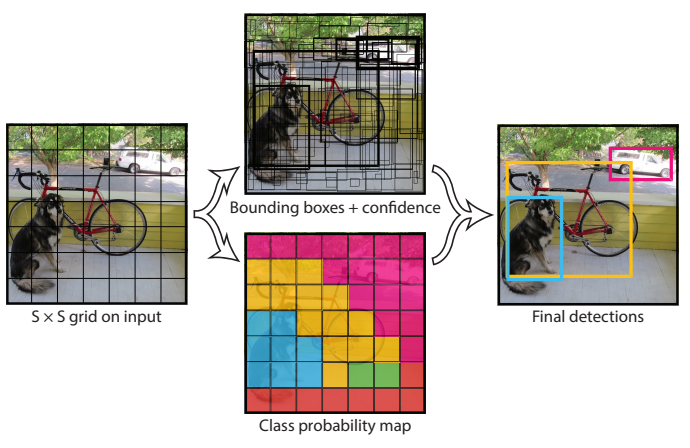
\includegraphics[width=\linewidth]{images/00_YOLO.PNG}
 
\section{Introduction}
 \quad real-time object detection model의 필요성에는 자율 주행 시스템처럼 실시간으로 이미지를 처리해야하는 task에 사용하능하다는 점이다.
 이미 object detection에서 좋은 성능을 내고 있는 R-CNN 모델은 object가 있을법한 위치를 찾는 과정이 오래 걸리기 때문에 정확도는 좋을지 몰라도 real-time task에는
 맞지 않다. 따라서 이 논문에서는 R-CNN의 모델의 2-stage(localization and classification)를 하나로 합쳐서 single regression problem 관점으로 전환하여 
 image pixel에서 bounding box의 좌표,크기 그리고 class probabilities를 output으로 내는 network를 설계하였다. YOLO의 장점으로는 빠르다는 점과 prediction 과정에서
 전체 이미지를 보지 때문에 background가 R-CNN보다 작다는 점, 마지막으로 train dataset과 다른 natural image나 artwork같은 data에서도 상대적으로 높은 정확도를 얻을 수 있다.
 반면 단점으로는 정확도가 R-CNN보다 떨어진다는 점과 작은 object에 대해서 localization이 잘 되지 않는다는 점이 있다.

\section{Unified Detection}
\subsection{Network Design과 training}
\quad Network Design은 아래와 같다.\cite{youtube}
\newline  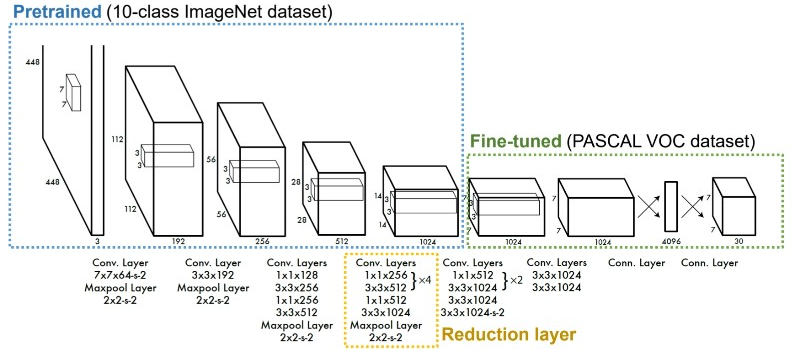
\includegraphics[width=\linewidth]{images/01_YOLO.PNG}
GoogLeNet 구조를 기반으로 24개의 convolution layer과 2개의 Fully connected layer로 YOLO를 설계하였다. 파란색으로 칠한 부분인
20개의 convolution layer에서는 1000-class ImageNet dataset으로 pre-training된 모델을 사용하였고 나머지 layer(4 conv.layer and 2 fc layer)
에서 PASCAL VOC dataset을 이용해서 fine-tuned을 진행하였다. fine-tuned network 시에 448x448 input image를 사용한 것은 resolution을 높여서
fine-grained visual information을 얻기 위해서이다. 또한 GoogLeNet의 inception module를 대신하여 3 by 3 convolution layer의 앞부분에 
1 by 1 reduction layer를 사용하여 계산량을 줄었다. 간단하게 모델의 동작과정을 살펴보자. 
\newline  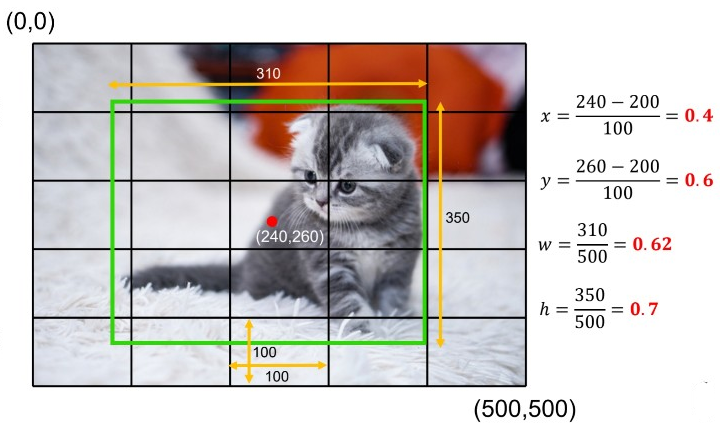
\includegraphics[width=9.5cm, height =5cm]{images/02_YOLO.PNG}
\newline 모델 설명을 위해서 단순한 가정을 해보자. input image가 500x500이고 cell을 5x5 grid cell로 나누었다는 가정이다. 이렇게 되면 그림 오른쪽에 적혀 있는 것처럼
x,y,w,h를 구할 수 있다. 여기서 x,y는 bounding box의 중심으로부터 grid cell 범위에 대한 상대 값이다. w,h는 현재 bounding box의 전체 이미지에 대한 상대값이다. 
여기에 confidence을 더해 총 2개의 box인 x,y,w,h,confidence와 class probability 20개를 가지고 output channel 수가 30개가 되도록 final layer을 설계한다.
실제로 YOLO 모델은 7x7 grid cell로 나누고 2의 bounding box를 사용하고 20개의 class probabilities를 사용하여 output이 7x7x30 tensor이다. 
앞서 언급한 confidence가 의미하는 것은 $Pr(Object) \times IOU_{pred}^{truth}$ 을 말하는 것으로 만약 object가 cell에 존재하지 않는다면 0이다.
class probabilities의 경우는 $Pr(Class_i|Object)$으로써 confidence와 곱해서 class의 확률을 나타낼 수 있다. 
결국 CNN을 통해 2개의 bounding box가 출력되는데 만약 같은 object를 가리키고 있다면 IOU가 가장 높은 한개의 bounding box만 학습시키는 것이 정확도 측면에서 더 좋다.
그래서 threshold 값을 두어 그 값보다 크게 되면 같은 object를 Detection하고 있다고 보고 값을 0으로 만들어 준다. 이과정을 NMS(non-maximal suppression) algorithm이라고 한다. 그림으로 설명하자면 아래와 같다.
\newline  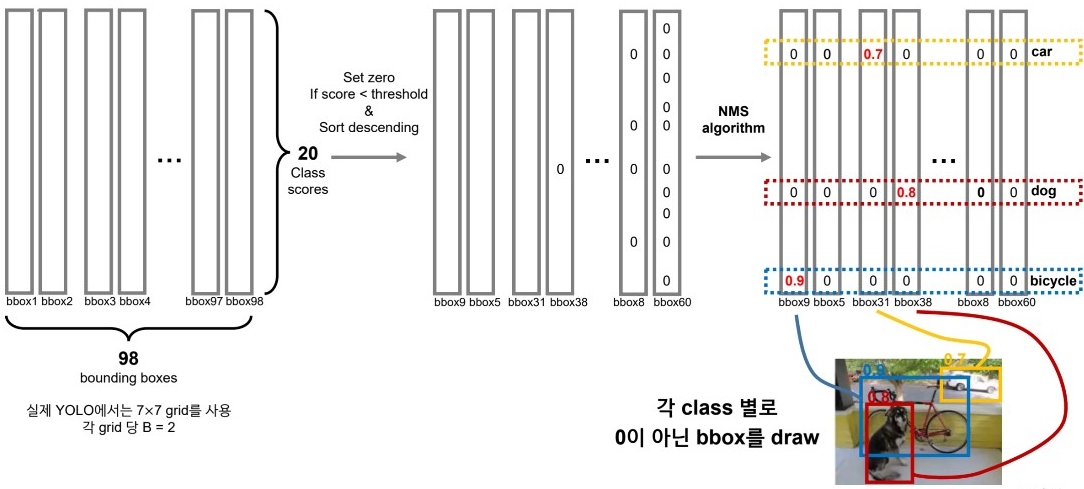
\includegraphics[width=\linewidth]{images/04_YOLO.PNG}
 YOLO 모델을 training 시킬 때는 leaky ReLU를 사용하였고 learning rate도 적절히 epoch을 끊어서 조절해주었다. 
또한, batch size을 64로 momentum을 0.9로 decay를 0.0005로 주었다. 그리고 overfitting을 막기 위해서 dropout과 data augmentation도 구현하였다.

\subsection{Loss function}
\quad object detection task를 regression 문제로 전환하기 위해 가장 중요한 것이 loss function이다. 먼저 sum-squared error을 사용하였는데
localization과 classification error에 대한 동일한 가중치를 둔다는 점과 background에 속하는 grid cell의 경우 confidence score이 0이 되도록 학습하는데 
이 과정에서 object를 포함하는 cell은 overpowering하게 만든다는 점이 문제점이 되었다. 그래서 아래와 같이 loss function을 새로 설계하였다.
\newline  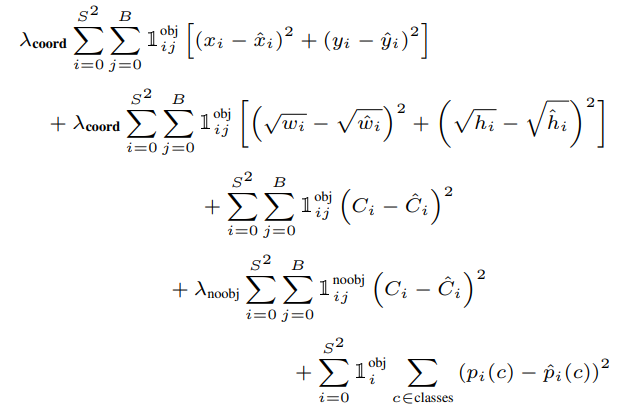
\includegraphics[width=\linewidth]{images/03_YOLO.PNG}
$1^{obj}_i$ 은 i번째 cell에 object가 있는지를 나타낸다. 
$1^{obj}_{ij}$ 는 i cell에서 j번째 bounding box predictor가 responsible한지를 나타낸다.
이 때 responsible이란 한 object를 누가 더 잘 detection하는지를 의미하는 표현이다.
여기서 w,h에 root를 사용한 것은 작은 object여도 큰 object와 별 차이없는 loss를 주기 위해서이다. 
2번째 줄까지의 식은 모든 grid cell에서 예측한 B개의 bounding box의 좌표와 ground truth 사이의 coordinate loss이고
3,4번째 줄은 모든 grid cell에서 예측한 confidence score과 ground truth사이의 confidence score loss이다.
5번째 줄은 conditional class probability 예측 값과 ground truth사이의 conditional class probability loss를 의미한다.

\section{Experiment}
\quad Deformable parts models(DPM)은 sliding window 방식으로 정적인 feature추출과 region 분류 등을 위해 분리된 pipeline을 사용하는 모델로
YOLO가 더 빠르고 정확도도 높다. R-CNN의 YOLO을 비교하자면 각각의 grid cell에서 CNN을 이용해서 bounding box와 score을 뽑는다는 공통점이 있는데 localization과 classification의
pipeline 하나인지 두개인지에 따라서 one-stage, two-stage로 나뉜다.
아래 실험결과를 보면 알수 있다시피 YOLO 모델이 다른 모델에 비해 압도적으로 FPS가 높고 정확도도 R-CNN에 비해 많이 뒤지지는 않는다.
\newline  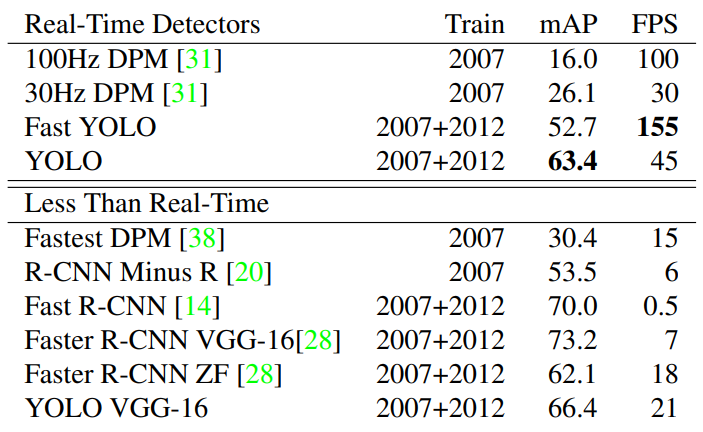
\includegraphics[width=9.5cm, height =5cm]{images/05_YOLO.PNG}
\newline 아래 그림은 Fast R-CNN과 YOLO을 비교한 것으로 R-CNN은 background error의 아쉬움이 있고 YOLO의 경우에는 localization의 아쉬움이 있다.
\newline  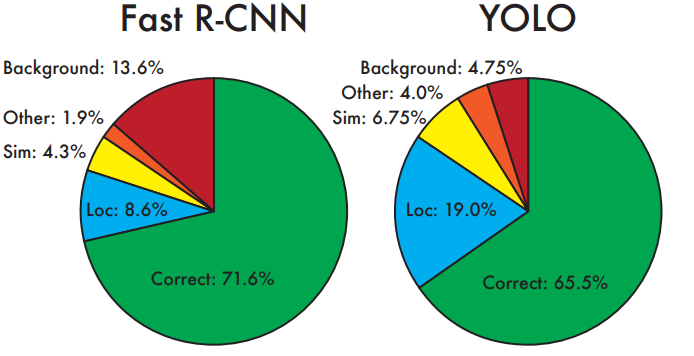
\includegraphics[width=9.5cm, height =5cm]{images/06_YOLO.PNG}
\newline 따라서 두 모델을 ensemble하게 되면 각각의 단점을 보안하여 Fast R-CNN보다 mAP가 3.2\%가 증가한 75\%의 정확도를 얻을 수 있었다. 
그외 결과에도 YOLO model의 경우에는 train data set과 distribution이 다른 dataset에서도 정확도 감소 정도 다른 모델에 비해 작았다. 이로 볼 때 YOLO가 
전체 이미지를 받아서 학습을 시키기 때문에 더 global한 feature을 학습한 것으로 추측한다. artwork dataset의 경우에서는 다른 모델에 비해 
압도적으로 AP가 더 높았다. 
\newline  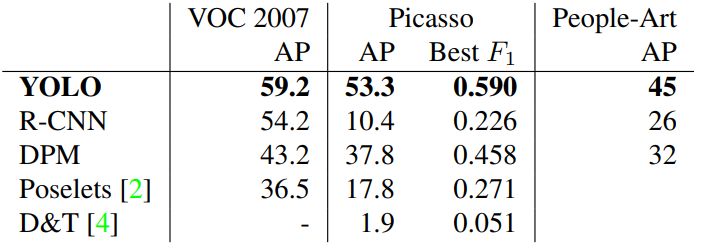
\includegraphics[width=9.5cm, height =3cm]{images/07_YOLO.PNG}

\section{Conclusion}
\quad 이 논문에서는 object detection model로써 paradigm을 바꾼 one-stage detector YOLO을 제시함으로써 object detection은 
두 가지 model로 발전하고 있다.\cite{h} YOLO는 비교적 높은 정확도를 가지면서 real-time video 분석에 사용할 수 있고 
심지어 natural data의 train dataset과 다른 distribution에서도 높은 정확도를 추출하기 때문에 매우 유용하다. 
또한 ene-to-end training이 가능하여 다루기도 쉽다.
\newline  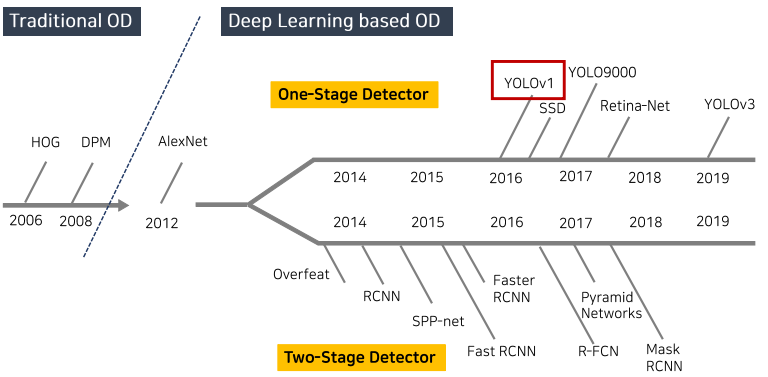
\includegraphics[width=\linewidth]{images/08_YOLO.PNG}

\newpage
\bibliography{egbib}

\end{document}